\subsubsection{Specifying boundary crossing probabilities in \texttt{gsDesign()}}

We use the CAPTURE example, working with the desired 80\% power ($\beta=.2$) to demonstrate deriving bounds with specified boundary crossing probabilities. 
For simplicity, we will let $\alpha_i^+(0)=.025/4$ and $\beta_i(\delta)=.2/4$, $i=1,2,3,4$. 
Setting the \texttt{gsDesign()} parameters \texttt{sfu} and \texttt{sfl} to \texttt{sfLinear}, the vector \texttt{p} below is used to equally allocate the boundary crossing probabilities for each analysis.
Note that \texttt{sfLinear()} requires an even number of elements in \texttt{param}.
The first half specify the timepoints using an increasing set of values strictly between 0 and 1 to indicate the proportion of information at which the spending function is specified.
The second half specify the proportion of total error spending at each of these points.
(Aside: those interested in plotting with special characters note the special handling of the character + in the argument \texttt{main} to \texttt{plot()}.) 
\bigskip

\begin{verbatim}
# Cumulative proportion of spending planned at each analysis
# In this case, this is also proportion of final observations at each interim
p <- c(.25, .5, .75)
t <- c(.25,.5,.75)
# Cumulative spending intended at each analysis (for illustration)
p * 0.025
n.fix <- nBinomial(p1=.15, p2=.1, beta=.2)
x <- gsDesign(k=4, n.fix=n.fix, beta=.2, sfu=sfLinear, sfupar=c(t,p),
              sfl=sfLinear, sflpar=c(t,p))
plot(x, main=expression(paste("Equal ", alpha[i]^{"+"}, (0), " and ", 
beta[i](delta), " for each analysis")))
x

\end{verbatim}
\bigskip


The printed output from the above is shown below and a plot of the derived boundaries is in Figure \ref{fig:sfPoints}. 
The columns labeled \texttt{Spend+} and \texttt{Spend++} show the values $\beta_i(\delta)$ and $\alpha_i(0)$, respectively, are equal for each analysis, $i=1,2,3,4$.
The nominal p-values for the upper bound increase and thus the bounds themselves decrease for each analysis.
That equal error probabilities results in unequal bounds is because of the correlation between the test statistics used for analysis that was indicated in (\ref{CanonicalCov}).
Note that the requirement of 1372 patients for the fixed design has now increased to a maximum sample size of 1786 which is an inflation of 30\%.
On the other hand, the expected number of patients when a boundary is crossed is 770 under the assumption of no treatment difference and 1054 under the alternative hypothesis of a 15\% event rate in the control group and 10\% in the experimental group.
Thus, this redesign seems reasonably effective at controlling the sample size when the experimental regimen has no underlying benefit.
The nominal $\alpha-$level of .0124 required for a positive result at the end of the study is almost exactly half that of the overall .025 for the study.
We will propose other designs that will not require such a small final nominal $\alpha$ by setting higher early efficacy bounds.
\bigskip

\begin{verbatim}
Asymmetric two-sided group sequential design with 80 % power and 2.5 % Type I Error.
Upper bound spending computations assume trial continues if lower bound is crossed.

                  ----Lower bounds----  ----Upper bounds-----
  Analysis   N    Z   Nominal p Spend+  Z   Nominal p Spend++
         1  447 -0.05    0.4816   0.05 2.50    0.0063  0.0063
         2  893  0.82    0.7953   0.05 2.41    0.0080  0.0063
         3 1340  1.53    0.9370   0.05 2.32    0.0101  0.0063
         4 1786  2.24    0.9876   0.05 2.24    0.0124  0.0062
     Total                      0.2000                 0.0250 
+ lower bound beta spending (under H1): Piecewise linear spending function with 
line points = 0.25 0.5 0.75 0.25 0.5 0.75
++ alpha spending: Piecewise linear spending function with 
line points = 0.25 0.5 0.75 0.25 0.5 0.75

Boundary crossing probabilities and expected sample size assuming any cross stops the trial

Upper boundary (power or Type I Error)
          Analysis
   Theta      1      2      3      4  Total   E{N}
  0.0000 0.0063 0.0062 0.0059 0.0042 0.0225  769.7
  0.0757 0.1843 0.2805 0.2253 0.1100 0.8000 1054.1

Lower boundary (futility or Type II Error)
          Analysis
   Theta      1      2      3      4  Total
  0.0000 0.4816 0.3321 0.1299 0.0339 0.9775
  0.0757 0.0500 0.0500 0.0500 0.0500 0.2000
\end{verbatim}

\begin{figure}
\begin{center}
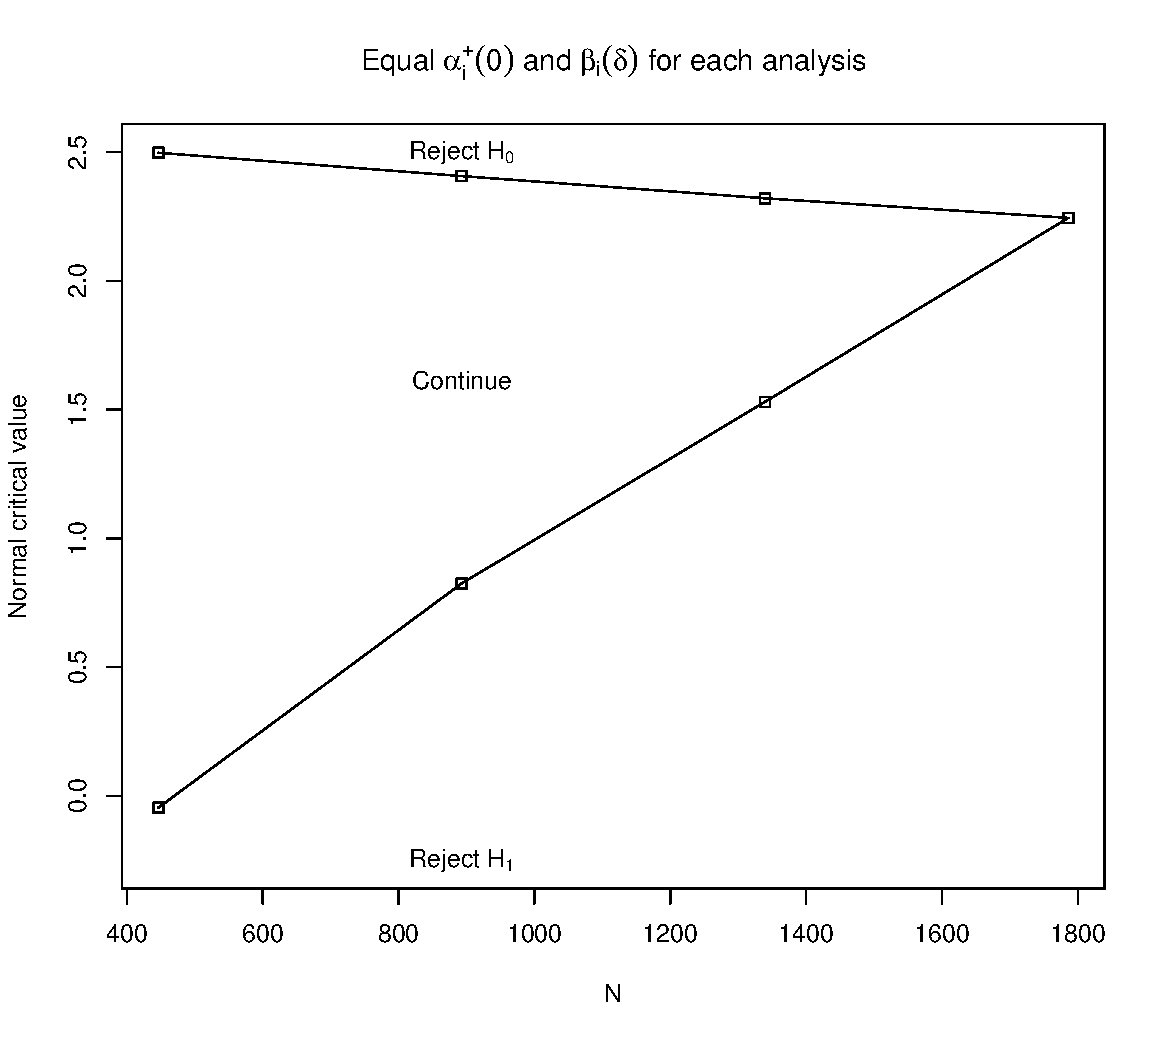
\includegraphics[width=.6\textwidth]{figs/boundplot2.pdf}
\end{center}
\caption{Boundary plot with equal $\alpha_i^+(0)$ and $\beta_i(\delta)$, $i=1, 2,3,4$.\label{fig:sfPoints}}
\end{figure}

Now we display piecewise linear spending functions. The plot resulting from the code below is in \ref{fig:sfLinear}.
\begin{verbatim}
# Cumulative proportion of spending planned at each analysis
# Now use a piecewise linear spending
p <- c(.05, .2, .5)
p2 <- c(.6,.8,.85)
x <- gsDesign(k=4, n.fix=n.fix, beta=.2, sfu=sfLinear, sfupar=c(t,p),
              sfl=sfLinear, sflpar=c(t,p2))
plot(x, plottype="sf", main="Piecewise linear spending")
\end{verbatim}

\begin{figure}
\begin{center}
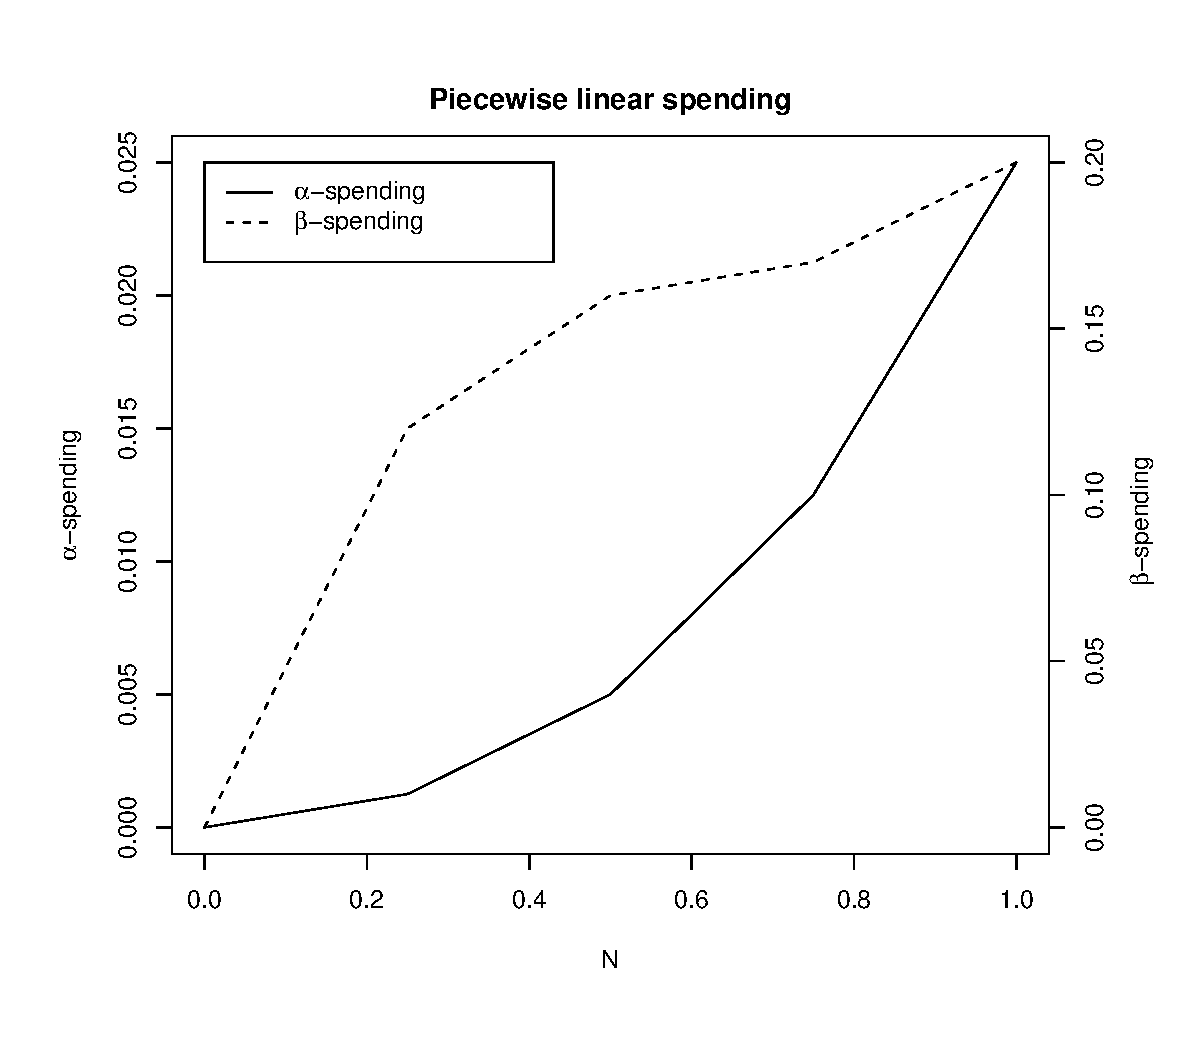
\includegraphics[width=.6\textwidth]{figs/sfLinear.pdf}
\end{center}
\caption{Piecewise linear spending functions.\label{fig:sfLinear}}
\end{figure}

